\chapter{Systém PerfEval}

Když už jsou známy požadavky na aplikaci, tak je možné začít ji navrhovat.
V~této kapitole jsou podrobně popsány úvahy a~rozhodnutí, které byly v~průběhu vývoje
provedeny. Jednotlivá rozhodnutí byla následně promítnuta do~architektury a~chování aplikace.

%\section{???}
%Výsledky testování výkonu se tedy musejí vyhodnocovat tak, že se podrobně prozkoumá výsledná sada čísel.
%Oproti testování korektnosti, kdy test projde nebo neprojde, je testování výkonu výrazně složitější.
%Pohledem na samostatnou sadu dat se nedá určit, zdali je software dostatečně rychlý. Aby bylo možné
%ze~sady určit něco vypovídajícího, bylo by možné stanovit pevný limit výkonnosti.
%Tento přístup nemusí být vypovídající při dlouhodobém vývoji
%a~při hodnotách hluboko pod limitem. Proto je vhodné, aby se datové sady, které testovací framework produkuje,
%porovnávaly mezi sebou. Porovnáním sad je totiž možné zjistit, jestli nedošlo k~významným změnám výkonu
%při~vývoji od~předchozí verze. Frameworky samotné však tuto možnost obvykle nemají.

\section{Analýza řešení}

\subsection{Měření výkonu}

Před začátkem vývoje PerfEvalu bylo nutné zamyslet nad tím, jak můžou výsledky měření výkonu softwaru vypadat.
V následujících odstavcích budou zmiňovány jednotlivé poznatky o~výsledcích měření výkonu.
Tyto poznatky vedly k~tomu, jak se PerfEval chová a~jakou má architekturu.

\medskip

\noindent\textbf{Měřené veličiny.} Jak jsme v první kapitole viděli, tak měřící
frameworky umožňují měřit mnoho různých fyzikálních veličin. Patří mezi ně například
doba vykonávání metody, frekvence počtu operací za jednotku času a spotřeba paměti.
Předpokládat se tedy dá jen to, že pokud vezmu dva výsledky měření výkonu ze~dvou různých
verzí, tak budou reprezentovány stejnou fyzikální veličinou a~v~lepším případě budou mít
i~stejnou fyzikální jednotku. Je tedy vhodné, aby výsledný systém byl schopen přijmout
jakoukoli veličinu bez ohledu na jednotku.

\medskip

\noindent\textbf{Identifikátory testů.} Protože testovací frameworky nepoužívají žádné identifikátory testů, tak je nejpřímější
řešení k~jejich rozpoznávání používat jména testovacích metod jako identifikátor. Tato jména poskytují ve~výsledcích
měření jak framework BenchmarkDotNet, tak framework JMH. Z~dokumentace frameworku Criterion \cite[]{criterion}
pro měření výkonu v~jazyce~Rust se název metody ve~výsledcích nachází také. Z~toho lze
usoudit, že použití jména metody jako identifikátoru může být dostatečně obecné.

\medskip

\noindent\textbf{Kompilace just-in-time.} V~případě měření výkonu u~jazyků, které jsou kompilované metodu JIT, je nutné být obezřetný. Je nutné
všímat si, jaká data byla naměřena. Jazyky kompilované metodou JIT mohou při měření podléhat tzv. zahřívací
fázi. Jedná se o~fázi, kdy kód ještě není plně optimalizovaný, ale již se provádí a~může být měřen.
V~závislosti na použitém měřícím frameworku je pak nutné naměřená data vhodně filtrovat. V~případě, že
by se data před a~po~optimalizaci nacházela v~jedné sadě dat, mohla by být zkreslená.

\subsection{Použití statistických metod pro analýzu dat}

\noindent\textbf{Výsledek měření.} S~testováním výkonu je problém. Když se spustí měření výkonu, tak výsledkem je pouhá
datová sada. Tato datová sada nevypovídá nic o~změně průběžného výkonu, která
je zajímavá. Právě podle změny ve~výkonu softwaru je možné zjistit, jestli je nutné
kód optimalizovat, protože dochází k~významným zhoršením.

\medskip

\noindent\textbf{Šum.} Při měření výkonu dochází jako při jakémkoli jiném měření k šumu. Tento šum se projevuje
tak, že pokud se měření opakuje při~stejných podmínkách, tak se naměřené hodnoty liší.
Tomuto šumu se nelze vyvarovat. Měření proto opakujeme a~naměřené hodnoty vyhodnocujeme
pomocí statistických metod, které si s~tímto šumem poradí.

\medskip

\noindent\textbf{Testování hypotéz.} Pro vyhodnocování výkonu je využito metod testování hypotéz. Ve statistickém testování
hypotéz se snažíme zamítnout nulovou hypotézu. V~případě zamítnutí nulové hypotézy
se předpokládá, že platí alternativní hypotéza. Popis testování hypotéz v této kapitole
se řídí skripty Pravděpodobnost a~statistika~1 \cite[]{samal_nmai059_nodate}.

Při testování hypotéz rozeznáváme
chyby I. a~II. druhu. Chyba I. druhu znamená, že jsme nulovou hypotézu zamítli,
i~když platí. Chyba II. druhu znamená, že jsme ji nezamítli, ale ona neplatí.

V našem případě porovnávání výkonu bude nulová hypotéza tvrzení, že výkon dvou verzí softwaru je stejný.
Jako alternativní hypotézu budeme uvažovat, že výkony dvou verzí softwaru jsou různé.
Pomocí metody testování hypotéz bude zjišťováno jestli mají dvě spojité náhodné veličiny stejnou střední hodnotu.
Hodnoty spojité náhodné veličiny jsou vždy hodnoty výkonu jedné testované metody programu jedné z verzí.
Pro každou z verzí je tedy uvažovaná jedna náhodná veličina.
Pokud hodnoty těchto veličin mají stejnou střední hodnotu, tak budeme tvrdit, že i výkon obou porovnávaných
verzí je stejný.

Chyba I. druhu tedy v našem případě znamená, že jsme prohlásili, že výkony dvou verzí jsou různé,
ačkoli jsou stejné. Pravděpodobnost chyby I. druhu je obvyklý parametr statistického testu.
Pravděpodobnost chyby I. druhu bude dále značen jako parametr $\alpha$. Parametr $\alpha$
je součástí konfigurace systému PerfEval.

Následující dvě podkapitoly popisují vybrané statistické testy, které jsou využity v~systému PerfEval.
Dvouvýběrový Welchův t-test byl vybrán, protože t-test se podle \cite[]{samal_nmai059_nodate} používá pro porovnání
středních hodnot dvou náhodných veličin. Welchův t-test byl vybrán, protože oproti Studentovu t-testu nevyžaduje
stejné rozptyly porovnávaných náhodných veličin. Percentilový hierarchický bootstrap byl vybrán, protože
je vhodný v~situaci, kdy není možné předpokládat normální rozdělení dat.
Poslední podkapitola popisuje jakým způsobem se řeší nevyvrácení nulové hypotézy.

\subsubsection{Welchův dvouvýběrový t-test}

Welchův dvouvýběrový t-test se používá jako testová statistika při testování hypotéz.
Tato statistika předpokládá, že náhodné veličiny jsou nezávislé a jejich rozdělení
se blíží normálnímu rozdělení. Nezávislost náhodných veličin je dána vlastnostmi
experimentu \cite[]{twosampletests} a její zajištění je mimo doménu řešeného problému. PerfEval
tedy v~případě použití možnosti t-test možnou závislost zanedbává.

Normalitě náhodných veličin je možné se přiblížit díky centrální limitní větě (CLV).
Se zajištěním normality nám pomůže samotná struktura naměřených výsledků. Výsledky měření
obsahují běhy. Běhy obsahují jednotlivé naměřené hodnoty. Naměřené hodnoty představují
vzorky náhodné veličiny. Pokud se budou v~rámci t-testu namísto naměřených hodnot uvažovat
průměry jednotlivých běhů, tak se podle CLV bude rozdělení těchto průměrů blížit normálnímu rozdělení.

Interval spolehlivosti pro Welchův t-test se spočítá podle dále uvedených vzorců.
Postupně se počítají stupně volnosti, kritická hodnota t-rozdělení, chybovost, dolní a~horní mez intervalu.
Vzorec pro výpočet stupňů volnosti je převzatý z~Wikipedie Welchova t-testu \cite[]{enwiki:1184251732}.
Ostatní vzorce jsou převzaty ze skript \cite[]{samal_nmai059_nodate}.

\begin{equation*}
    \bar{X_i} = \frac{1}{n_i} \sum_{j=1}^{n_i} X_{ij}
\end{equation*}

\begin{equation*}
    s_i^2 = \frac{1}{n_i-1} \sum_{j=1}^{n_i} (X_{ij} - \bar{X_i})^2
\end{equation*}

\begin{equation*} \label{eq:welch_df}
    df = \frac{(\frac{s_1^2}{n_1} + \frac{s_2^2}{n_2})^2}{\frac{s_1^4}{n_1^2(n_1-1)} + \frac{s_2^4}{n_2^2(n_2-1)}}
\end{equation*}

\begin{equation*}
    t = \psi_{df}^{-1}(1-\frac{\alpha}{2})
\end{equation*}

\begin{equation*}
    marginOfError = t \cdot \sqrt{\frac{s_1^2}{n_1} + \frac{s_2^2}{n_2}}
\end{equation*}

\begin{equation*}
    lowerBound = \bar{X_1} - \bar{X_2} - marginOfError
\end{equation*}

\begin{equation*}
    upperBound = \bar{X_1} - \bar{X_2} + marginOfError
\end{equation*}

Použité značení:
\begin{itemize}
    \item $df$ - stupně volnosti
    \item $s_1^2$ - výběrový rozptyl první sady vzorků
    \item $s_2^2$ - výběrový rozptyl druhé sady vzorků
    \item $n_1$ - počet prvků první sady vzorků
    \item $n_2$ - počet prvků druhé sady vzorků
    \item $t$ - kritická hodnota t-rozdělení
    \item $\psi_{df}^{-1}$ - inverzní distribuční funkce t-rozdělení
    \item $\bar{X}_1$ - výběrový průměr první sady vzorků
    \item $\bar{X}_2$ - výběrový průměr druhé sady vzorku
\end{itemize}


%\begin{algorithm}[!ht]
%    \caption{WelchCI}
%    \KwIn{samples1, samples2, critValue}
%    \KwOut{lowerBound, upperBound}
%
%    n1 = length(samples1)\;
%    n2 = length(samples2)\;
%
%    mean1 = mean(samples1)\;
%    mean2 = mean(samples2)\;
%
%    var1 = var(samples1)\;
%    var2 = var(samples2)\;
%
%    varOverN1 = var1 / n1\;
%    varOverN2 = var2 / n2\;
%
%    degreesOfFreedom = Math.Pow(varOverN1 + varOverN2, 2) / (varOverN1 * varOverN1 / (N1-1) + varOverN2 * varOverN2 / (N2-2))\;
%
%    tDist = new TDistribution(degreesOfFreedom)\;
%    tCrit = tDist.inverseCumulativeProbability(critValue / 2)\;
%    marginOfError = tCrit * Math.Sqrt(varOverN1 + varOverN2)\;
%
%    lowerBound = mean1 - mean2 - marginOfError\;
%    upperBound = mean1 - mean2 + marginOfError\;
%
%\end{algorithm}

Nakonec se již jen zkoumá, zdali tento interval obsahuje nulu.
Pokud interval nulu neobsahuje, pak lze s~pravděpodobností $1-\alpha$ správně tvrdit, že
nulová hypotéza neplatí.

\subsubsection{Percentilový hierarchický bootstrap}

%% - https://www.youtube.com/watch?v=Xz0x-8-cgaQ

Bootstrap je statistická metoda využívající tzv. resamplování.
Stejně jako u~dvouvýběrového t-testu se předpokládá nezávislost náhodných veličin.
Podmínka nezávislosti bude zanedbána, protože ji není možné zaručit.
Bootstrap se jako metoda používá v~případě, kdy o~náhodných veličinách není možné
určit téměř žádné silné předpoklady. Díky této vlastnosti je bootstrap pro testování
hypotéz o~výkonu verzí softwaru použit.

\begin{algorithm}[!ht]
    \caption{MeanBootstrap1D}
    \KwIn{measurements, replicationCount}
    \KwOut{bootstrappedSamples}
    
    n = length(measurements)\;
    samples = []\;

    \For{i = 0; i < replicationCount; i += 1}{
        resampledSamples = []\;
        \For{j = 0; j < n; j = j + 1}{
            index = random() mod n\;
            resampledSamples.add(measurements[index])\;
        }
        samples.add(mean(resampledSamples))\;
    }
    
    \Return{samples}\;
\end{algorithm}

\begin{algorithm}[!ht]
    \caption{MeanBootstrap2D}
    \KwIn{runs1, runs2, replicationCount}
    \KwOut{bootstrappedSamples}
    
    n = length(runs1)\;
    m = length(runs2)\;
    samples = []\;
    
    \For{i = 0; i < replicationCount; i += 1}{
        samples1 = []\;
        \For{j = 0; j < n; j += 1}{
            index = random() mod n\;
            samples1.add(MeanBootstrap1D(runs1[index], 1))[0]\;
            }
        samples2 = []\;
        \For{k = 0; k < m; k += 1}{
            index = random() mod m\;
            samples2.add(MeanBootstrap1D(runs2[index], 1))[0]\;
        }
        diff = mean(samples1)-mean(samples2)\;
        samples.add(diff)\;
    }
    
    \Return{samples}\;
\end{algorithm}

Podle percentilového bootstrapu se interval spolehlivosti nalezne tak, že se hranice intervalu stanoví jako $\frac{\alpha}{2}$-tý
a~$\frac{1-\alpha}{2}$-tý percentil z~resamplovaného souboru. Tyto dvě hodnoty budou představovat hranice intervalu.

Zkoumanou náhodnou veličinou je rozdíl dvou náhodných veličin. Tyto dvě náhodné veličiny jsou dány měřením
výkonnosti dvou verzí softwaru. Nulová hypotéza, která je vyvracena, tvrdí, že obě veličiny mají stejnou střední hodnotu.
Pokud tedy interval spolehlivosti neobsahuje nulu, tak můžeme nulovou hypotézu vyvrátit, protože s~pravděpodobností
$1-\alpha$ o ní test správně prohlásil, že neplatí.

Naměřené vzorky však nejsou prostý statistický soubor. Jedná se o~hierarchický soubor dat.
Každé jedno měření se skládá z~jednoho, nebo více běhů. Každý běh se skládá z~jednoho, nebo více naměřených údajů.
Vytváření bootstrapového statistického souboru tedy vypadá trochu odlišně.

MeanBootstrap2D ukazuje, jak vypadá výběr nového statistického souboru. Vyberou
se náhodné běhy z~jednotlivých výsledků měření. Z~těchto běhů se získá 1D bootstrap.
Novým prvkem vytvářeného statistického souboru se stane rozdíl těchto bootstrapů.

\subsubsection{Co dělat v případě nevyvrácení hypotézy?}

V~případě nevyvrácení nulové hypotézy nám statistické testy nedávají žádnou informaci.
I~přes tuto vlastnost statistických testů, je pro praktické užití nutné se rozhodnout, zdali
změnu výkonu hlásit. Stále je nutné se vyvarovat chyby II. druhu. Proto v~tomto případě nebudeme hlásit zhoršení výkonu,
pokud bude získaný interval spolehlivosti dostatečně úzký. Pokud má tedy interval spolehlivosti
dolní mez $D_{LOW}$ a horní mez $D_{HIGH}$, pak je jeho šířka $D_{HIGH}-D_{LOW}$. Odhadovaný průměr by byl $\frac{D_{HIGH}+D_{LOW}}{2}$.
Relativní šířka intervalu je tedy poměr šířky a průměru, tedy $\frac{2\cdot(D_{HIGH}-D_{LOW})}{D_{HIGH}+D_{LOW}}$.

V případě většího množství vzorků je možné zužovat interval spolehlivosti. Vztah mezi
šířkou a~počtem vzorků odpovídá $O(\frac{1}{\sqrt{n}})$, kde $n$ je počet vzorků. Z~daného
množství vzorků je tedy možné odhadnout, kolik vzorků je ještě zapotřebí změřit.

V~případě, že je interval dostatečně úzký, nebudeme zhoršení výkonu hlásit a~řekneme, že výkon obou verzí je stejný.
V~případě, že interval není dostatečně úzký, prohlásíme, že vzorků není dost.

PerfEval tedy v~konečném důsledku rozlišuje tři základní výsledky porovnání výkonu verzí.
Test nahlásí zhoršení výkonu právě tehdy, když bude nulová hypotéza vyvrácena a~zároveň
bude průměrný výkon novější verze horší než průměrný výkon starší verze.
Test nenahlásí žádnou změnu výkonu, pokud nulová hypotéza nebyla vyvrácena a~interval spolehlivosti
bude dostatečně úzký. V~případě, že nulová hypotéza nebyla vyvrácena a~interval spolehlivosti
je příliš široký, test nahlásí, že vzorků není dostatečné množství.

\subsection{Použité statistické metody}
Pro porovnání dvou výsledků měření se používají statistické metody. Statistické metody se používají k~zjištění,
jestli výsledky měření považované za~náhodné veličiny mají stejnou střední hodnotu a~jestli je vzorků dostatečné množství.
V~předchozí kapitole byly popsány dvě statistické metody, které jsou v~systému PerfEval implementovány.
Jedná se o~metody \textbf{bootstrap} a~\textbf{t-test}.

\medskip

\noindent\textbf{Bootstrap.} Výhodou bootstrapu je, že není vyžadovaný předpoklad normálního rozdělení dat.
Bootstrap je implementován pomocí algoritmů z~předchozí podkapitoly. Je tedy patrné, že výpočet je pomalý,
protože dochází k~velkému množství náhodných výběrů z~dvoudimenzionální sady dat. Pokud má uživatel
dostatečné množství času měl by této metodě dát přednost právě kvůli tomu, že není vyžadován předpoklad normálního rozdělení dat.
Jak již bylo řečeno, tak zajištění normality dat je totiž mimo doménu řešeného problému.

\medskip

\noindent\textbf{T-test.} T-test je použitý ve variantě Welchova t-testu. Tento test je výhodný tím, že je rychlejší než bootstrap.
Rychlejší je proto, že se jedná o pouhé dosazení hodnot do vzorců. Nevýhodou je, že je vyžadován předpoklad normálního rozdělení dat.
Tento předpoklad však není zaručen, a tudíž může dojít k~zkreslení výsledků. T-test je tedy vhodný pro případy, kdy je množství naměřených
vzorků velké a~uživatel má málo času na~vyhodnocení výsledků.

\subsection{Spouštění testů systémem PerfEval}
V~počátku vývoje bylo nutné se~rozhodnout, jakým způsobem bude systém přijímat a~zpracovávat výsledky testů.
V~úvahu přicházela varianta \textbf{Měření výkonu uživatelem}, že~uživatel provede měření výkonu sám. Druhá varianta byla \textbf{Měření výkonu PerfEvalem} tak,
že~uživatel systému vysvětlí, jakým způsobem se~testování výkonu spouští. Pokud by byla zvolena tato varianta,
tak by bylo nutné nalézt dostatečně univerzální způsob spouštění testů.

\medskip

\noindent\textbf{Měření výkonu PerfEvalem.} Aplikace a~benchmarky pro měření výkonu mohou být jak konzolové, tak grafické aplikace. Pokud by PerfEval měl
měření provádět sám, tak by téměř určitě nebyl schopen pracovat s~grafickými aplikacemi, ale byl by schopen
spouštět programy s~parametry na~příkazové řádce.

Dále by bylo nutné vysvětlit, jak vypadá výstup spouštěných testů. Když pomineme formát, tak je nutné zjistit,
kam program, který provádí měření, výsledky ukládá. Benchmarkovací systém BenchmarkDotNet například vypisuje
výsledky měření v podobě tabulky na standardní výstup a~zároveň ukládá strojově čitelné výsledky do~speciálního
k~tomu určeného adresáře.

Pokud by PerfEval využíval této varianty, tak by uživatel při inicializaci systému musel zadat, jak spustit testy
a~kam se uloží výsledek. Tímto způsobem by došlo k~tomu, že PerfEval by začal určovat, jak mají vypadat programy,
jejichž výstupy přijímá.
\medskip
\noindent\textbf{Měření výkonu uživatelem.} V této variantě tedy uživatel spouští testy sám a~PerfEval pouze porovnává výsledky.
Při inicializaci uživatel oproti předchozí variantě pouze vybere vhodný parser. Zvolený parser umí zpracovat příslušný formát dat z~benchmarkovacího frameworku,
který uživatel používá. Toto řešení bylo vybráno a~implementováno v~systému PerfEval.

Vybrané řešení tedy od uživatele požaduje krok navíc. Nicméně dává uživateli mnohem větší prostor pro to, jak
spouští testy a~kam ukládá výsledky. O~tom, že existují výsledky měření dané verze, a kde se nachází, uživatel
pouze informuje PerfEval. Systém tak ani do budoucna neklade žádné nároky na to, jak má uživatel testy spouštět,
ani kde se mají výsledky ukládat.

\subsection{Rozpoznání formátu výsledků měření}

Systém, který porovnává výsledky měření výkonu, by měl mít informace o~tom v~jakém formátu jsou data uložena
a~který benchmarkovací framework je vytvořil. Podle použitého frameworku a~formátu je totiž možné výsledky
měření zpracovat pomocí programu a~transformovat data o~měření tak, aby jim systém rozuměl.
Problém je tedy v tom, jak se systém dozví o~tomto formátu a~o~použitém frameworku.

Nejpříjemnější řešení pro uživatele by bylo, že by systém sám přišel na to, který framework a~formát je použitý.
Uživatel by totiž nemusel vědět pomocí jakého frameworku a~v~jakém formátu data ukládá. Pro systém by však mohl
být problém různé frameworky rozlišit.

Při rozlišování by se totiž musel podívat do~dat uložených v souboru
a~na~základě obsahu určit o~jaký formát a~framework se jedná. Správné určení frameworku a~formátu by bylo zásadní pro
správnou reprezentaci dat. Samotné rozlišování frameworků a~formátu by bylo obtížné, protože soubory s~výsledky
měření obsahují podobná data a~položky, ale hierarchie struktur ve~kterých jsou uloženy jsou různé.
Při následném rozlišování většího množství formátů a~frameworků by tedy systém automatického rozpoznávání
začal být příliš komplikovaný, aby si zachoval přesnost.

Docházelo by také k~dvojímu čtení souboru z~paměti. První čtení souboru by sloužilo k rozpoznání formátu,
aby systém zjistil, jak má data ze souboru zpracovávat. Při druhém čtení souboru by již transformoval data
tak, aby jim rozuměla vyhodnocovací část systému.

PerfEval tedy řeší tento problém tak, že uživatel při inicializaci zadá jméno jednoho z~dostupných parserů.
Předpokládá se tedy, že pokud uživatel používá výkonnostní testy, tak framework a~výstupní formát je shodný s~těmi které zvolený parser rozpoznává.
Pokud má PerfEval parser pro tento framework a~formát dat parser, pak je schopný vyhodnocovat výsledky měření.
V~opačném případě si tento parser může uživatel doimplementovat.

Tento přístup umožňuje snazší implementaci nových parserů. Není totiž nutné k těmto parserům implementovat
také sadu pravidel, kdy má být použitý. Uživatele tento přístup omezuje v tom, že musí znát framework a~formát
ve~kterém se výsledky měření nachází. Protože psaní výkonnostních testů není jednoduché, tak lze předpokládat,
že uživatel je dostatečně zkušený, aby tuto znalost měl.

\subsection{Kdy zpracovávat naměřená data?}

Systém musí v~některém bodě výpočtu zpracovat data z~měření. Existuje několik možností, kdy
je možné toto zpracování do formátu, kterému bude rozumět, udělat. Je možné buď zpracovat
data ihned po tom, co se systém dozví o~jejich existenci, nebo až těsně před vyhodnocováním.

Pokud by se data zpracovávala hned po tom, co se o nich systém dozví, tak to nutně neznamená,
že již má proběhnout vyhodnocování. Je tedy nutné zvolit nějaký formát do kterého zpracovaná data
uložit. Při vyhodnocení by se pak data z~tohoto formátu musela opět zpracovat. Tento způsob
zpracování dat by měl význam pouze v~případě, že by první předzpracování vedlo k~velkému
zrychlení druhého zpracování. Zároveň by toto řešení vedlo k~dvojímu ukládání dat, protože
by někde byl uložený původní výsledek měření v původním formátu, a~také soubor se~předzpracovanými
výsledky měření, který by obsahoval data se~stejným významem.

Výše zmíněné nevýhody vedly k tomu, že systém zpracovává data z~původního formátu těsně před
vyhodnocováním. Podle zvoleného parseru se tedy data naparsují těsně před vyhodnocením ze~souborů,
které vygeneroval přímo framework pro měření výkonu.

\subsection{Jak přistupovat k naměřeným datům?}

Systém, který porovnává výsledky měření, by měl mít nějaké informace o~tom, k~jaké verzi se měření vztahuje, nebo kde
se soubor s~výsledky nachází. Proto bylo při vývoji nutné se zamyslet nad tím, jakými způsoby lze tyto informace získat a~spravovat.
Systém PerfEval potřebuje o~výsledcích měření vědět, kde jsou uloženy a~ke~které verzi softwaru bylo měření provedeno.

\noindent\textbf{Složka s výsledky měření.} První zvažovaná varianta byla, že by existovala složka, do~které by uživatel vkládal výsledky měření. Tento adresář by byl určený
systémem PerfEval, nebo by byla zadaná cesta k~němu při inicializaci systému. Po~každém měření by tedy uživatel výsledek pouze
vložil do~správné složky a~o~nic víc by se nemusel starat.

Toto řešení má několik nevýhod. Omezuje uživatele v~tom, jak musí výsledky testů ukládat. Dále by se špatně určovalo,
ke~které verzi bylo měření provedeno, protože toto se ve~výsledcích měření běžnými frameworky neudává. Pravděpodobně by proto
vznikla hierarchie v tomto adresáři a~uživatel by například pomocí pojmenovávání složek určoval, ke~které verzi se měření vztahuje.

Celkově tedy tento způsob poskytuje jednoduché zjištění, kde se výsledek testu nachází. Je to pevně dané. Není ale možné jednoduše
zjistit verzi, protože je nutné projít adresářovou strukturu, což může být při velkém množství dat pomalé.

\medskip

\noindent\textbf{Cache a~složka s~výsledky měření.} Druhé uvažované řešení bylo vylepšení prvního řešení o~cache a sledování času modifikace adresářů.
Verze se totiž dobře určují při vkládání,
ale špatně dohledávají. Pravděpodobně by se používání některých verzí k~porovnání opakovalo častěji než u~jiných.
Zároveň pokud by nejnovější verze nebyla v cache, tak by se dohledávala postupným průchodem na základě nejmladšího data změny adresáře
v~adresáři s~výsledky měření. Cache by byla tvořena posledními několika desítkami naposledy použitých záznamů s~cestou k~výsledkům měření a~verzí.

Toto řešení má ale podobné nevýhody jako první. V~případě, že se verze porovnává poprvé, tak záznamy o~ní jistě nejsou v~cache
a~musí se prohledat adresářová struktura. Pokud je poslední úprava cache starší než nejnovější úprava nějakého podadresáře v~adresáři
s~výsledky měření, tak je nutné tuto část adresářové struktury projít. V~procházené části adresářové struktury je vždy nutné prozkoumat
zdali se jedná o~soubor verze, která je v cache, a~tak by se do ní měl přidat záznam o~tomto souboru. Popsaná práce s~cache měla
za~následek poslední uvažované řešení, kde již nezáleží na tom, kde jsou uložené výsledky měření. Jediné, co budeme předpokládat, je,
že uživatel soubory s~výsledky měření nepřesouvá.

\medskip

\noindent\textbf{Databáze s metadaty o~výsledcích měření.} Poslední uvažované řešení je strukturované ukládání metadat o~výsledcích měření. Využije se databáze o~jedné tabulce, kde
je uvedena cesta k~výsledku měření a~verze ke které byl výsledek změřen. Uživatel do~systému nahlásí, že má nový výsledek
měření, kde je uložen, a~k~jaké verzi softwaru je měření provedeno. Systém si tato data pouze poznamená do~databáze. Při
vyhodnocení pak pomocí databázových dotazů nalezen snadno všechny soubory s~výsledky měření k~potřebné verzi.

Toto řešení poskytuje jak rychlé vkládání nových výsledků, tak rychlé vyhledávání výsledků měření k~dané verzi.
Díky těmto vlastnostem bylo vybráno a~implementováno v~systému PerfEval.

\subsection{Formát výstupu}

Při volbě formátu v~jakém se budou výsledky výkonnostních testů prezentovat je nutné se zamyslet nad tím, kdo je bude číst a~zpracovávat.
Výsledky vyhodnocení bude zpracovávat zejména člověk a~průběžná integrace v~rámci verzovacího nástroje Git.

Pro člověka je čitelný formát zpracovaných dat tabulka s údaji o~tom, který test prošel a~který ne.
Jeden z~výstupních formátu systému PerfEval je takováto tabulka na příkazové řádce. Druhý formát s daty čitelnými pro člověka je
tabulka na HTML stránce, kterou PerfEval umí vygenerovat. Výstup v~HTML formátu je výhodný, protože je možné
soubor s~výsledky otevřít v~internetovém prohlížeči, který je dnes dostupný téměř na každém zařízení.

Strojem čitelný formát je XML soubor. XML má formát shodný s JUNIT XML formátem, který je běžně používaný v~průběžné integraci
při hlášení výsledků unit testů. Druhým zvoleným formátem je JSON, který je dnes běžně používaný pro serializaci dat v~různých
programovacích jazycích. Umožňuje tak snadnou integraci s dalšími programy.

\section{Architektura systému PerfEval}

Tato kapitola se věnuje popisu konkrétní architektury systému PerfEval.
Popisuje jakým způsobem jsou jednotlivé části systému navrženy a~jak spolu vzájemně interagují.

Samotné vyhodnocování jakožto porovnání dvou výsledků měření jedné sady testů výkonu je proces, který lze rozdělit do~několika kroků.
Zpracování dat uložených v souborech s výsledky měření až po vypsání výsledků vyhodnocení probíhá následujícím způsobem:

\begin{enumerate}
    \item Načtení a naparsování výsledků měření ze~souborů.
    \item Pomocí statistického testu porovnat dvě sady naměřených dat.
    \item Výsledek porovnání vypsat uživateli.
\end{enumerate}

\begin{figure}[!ht]
    \centering
    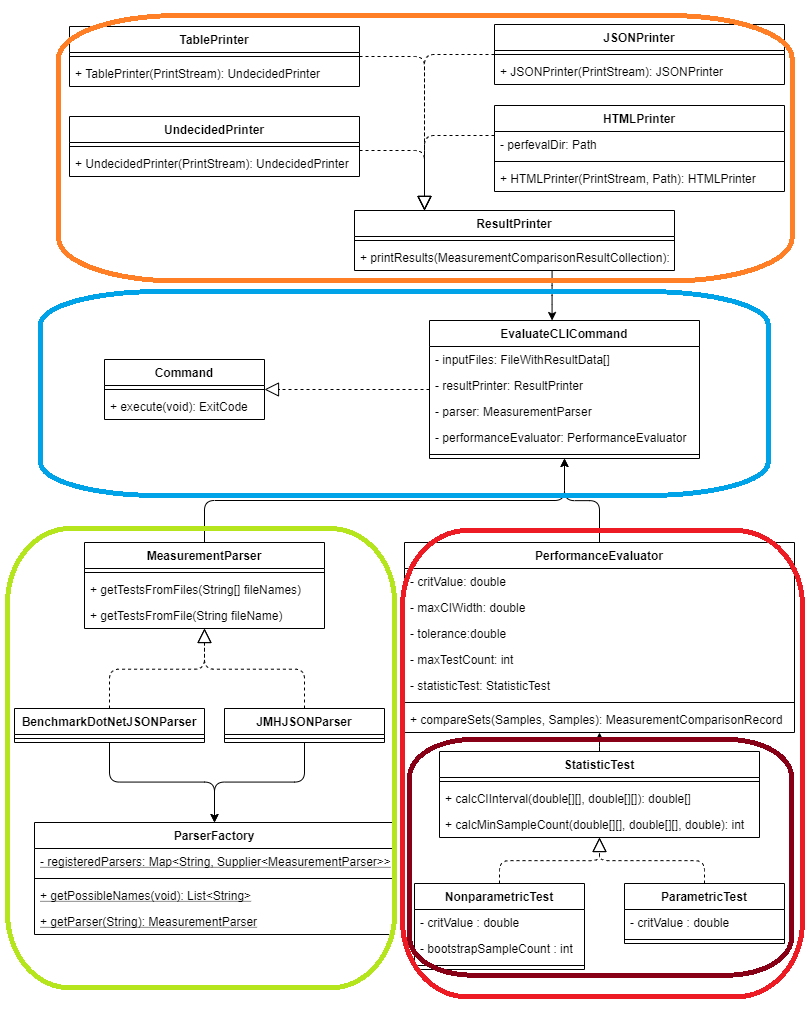
\includegraphics[width=0.92\textwidth]{../img/perfeval_evaluate_rect.png}
    \caption{Objektový návrh části PerfEvalu pro porovnávání výsledků měření}
\end{figure}

Obrázek 3.1 ukazuje rozdělení architektury vyhodnocovací části systému PerfEval do~čtyř logických celků.
Jedná se o logické celky, které se starají o~jednotlivé kroky vyhodnocování výsledků měření.

Na obrázku je vidět část systému kolem rozhraní \lstinline|MeasurementParser|, která se stará o~parsování výsledků měření.
Implementace tohoto rozhraní se stará o~načtení a~zpracování výsledků měření ze~vstupních souborů.
Produkují tak objekty, které reprezentují výsledky měření a~kterým rozumí zbytek systému.
Jednotlivé implementace tohoto rozhraní jsou závislé na~formátu výstupu frameworku, který byl použit pro měření výkonu.
Na základě konfigurace systému PerfEval vybere \lstinline|ParserFactory| správnou implementaci \lstinline|MeasurementParser|.

Obrázek dále znázorňuje třídu \lstinline|PerformanceEvaluator|, která se stará o~porovnání dvou instancí třídy \lstinline|Samples|.
Porovnání obstarává implementace rozhraní \lstinline|StatisticTest|. Volba implementace je dána parametry příkazové řádky.

Výsledky porovnání jsou následně vypsány uživateli pomocí implementace rozhraní \lstinline|ResultPrinter|.
Zvolená implementace tohoto rozhraní určuje formát výstupu, ve kterém jsou výsledky porovnání vypsány.
Volba implementace je dána parametry příkazové řádky.

Poslední částí, která je na obrázku 3.1 znázorněna, je hlavní třída celého vyhodnocování \lstinline|EvaluateCLICommand|.
Tato třída je implementací rozhraní \lstinline|Command|. Metoda \lstinline|execute| této třídy
provádí vyhodnocování podle popsaných kroků. Způsob provádění jednotlivých kroků je dané
dodanými implementacemi rozhraní \lstinline|MeasurementParser|, \lstinline|StatisticTest| a~\lstinline|ResultPrinter|.
Tyto implementace jsou předány při konstrukci třídy \lstinline|EvaluateCLICommand|.

Po vypsání výsledků porovnání se podle voleb z~konfiguračního souboru již jen nastaví exit kód programu a~ukončí se vyhodnocování.
Konfigurační soubor určuje jestli se mimo zhoršení výkonu hlásí také zlepšení výkonu a~nemožnost doměření dostatečného množství vzorků.

Samotná architektura systému je tedy postavena na rozhraních, které obklopují třídu \lstinline|EvaluateCLICommand|.
Pomocí nových implementací těchto rozhraní je možné systém rozšiřovat o~nové možnosti zpracování výsledků měření.
Architektura dále umožňuje snadné rozšíření o~nové formáty vstupu i~výstupu. Systém byl navržen tak, aby bylo
jednoduché změnit způsob provádění jednotlivých kroků vyhodnocování. Změna kroků samotných by vyžadovala
větší zásah do~architektury systému a~byla by složitá.


